\documentclass[dvipdfmx,a4paper,12pt]{article}
\usepackage[utf8]{inputenc}
%\usepackage[dvipdfmx]{hyperref} %リンクを有効にする
\usepackage{url} %同上
\usepackage{amsmath,amssymb} %もちろん
\usepackage{amsfonts,amsthm,mathtools} %もちろん
\usepackage{braket,physics} %あると便利なやつ
\usepackage{bm} %ラプラシアンで使った
\usepackage[top=30truemm,bottom=20truemm,left=25truemm,right=25truemm]{geometry} %余白設定
\usepackage{latexsym} %ごくたまに必要になる
\renewcommand{\kanjifamilydefault}{\gtdefault}
\usepackage{otf} %宗教上の理由でmin10が嫌いなので


\usepackage[all]{xy}
\usepackage{amsthm,amsmath,amssymb,comment}
\usepackage{amsmath}    % \UTF{00E6}\UTF{0095}°\UTF{00E5}\UTF{00AD}\UTF{00A6}\UTF{00E7}\UTF{0094}¨
\usepackage{amssymb}  
\usepackage{color}
\usepackage{amscd}
\usepackage{amsthm}  
\usepackage{wrapfig}
\usepackage{comment}	
\usepackage{graphicx}
\usepackage{setspace}
\usepackage{pxrubrica}
\usepackage{enumitem}
\usepackage{mathrsfs} 
\usepackage[dvipdfmx, bookmarks=false]{hyperref}
\setstretch{1.2}
\pagestyle{empty}

\newcommand{\mathsym}[1]{{}}
\newcommand{\unicode}[1]{{}}

\newcounter{mathematicapage}


%%%%%%%%% Theorem-like environment %%%%%%%%%%%
%
\theoremstyle{plain} %text of this environment is typesetted in italics
\newtheorem{theorem}{\indent\sc Theorem}[section]
\newtheorem{lemma}[theorem]{\indent\sc Lemma}
\newtheorem{corollary}[theorem]{\indent\sc Corollary}
\newtheorem{proposition}[theorem]{\indent\sc Proposition}
\newtheorem{claim}[theorem]{\indent\sc Claim}
\newtheorem{conjecture}[theorem]{\indent\sc Conjecture}
%
\theoremstyle{definition} %text of this environment is typesetted in roman letters
\newtheorem{definition}[theorem]{\indent\sc Definition}
\newtheorem{remark}[theorem]{\indent\sc Remark}
\newtheorem{example}[theorem]{\indent\sc Example}
\newtheorem{notation}[theorem]{\indent\sc Notation}
\newtheorem{assertion}[theorem]{\indent\sc Assertion}
\newtheorem{observation}[theorem]{\indent\sc Observation}
\newtheorem{problem}[theorem]{\indent\sc Problem}
\newtheorem{question}[theorem]{\indent\sc Question}
%
%If a theorem-like environment should not be numbered,
%add * after \newtheorem, and delete the counter option such as [theorem].
\newtheorem*{remark0}{\indent\sc Remark}
%
%%%%% Proof %%%%%
\renewcommand{\proofname}{\indent\sc Proof.}
%The following commands are available in the proof environment:
%\begin{proof}
%\end{proof}
%The end of a proof is marked with a square.
%%%%%%%%%%%%%%%%%%%%%%%%%%%%%%%%%%%%%%%%%

% -- enumerate, itemize行間設定
\usepackage{enumitem} % デフォルト設定
\setlist[itemize]{itemsep=3pt, parsep=0pt}
\setlist[enumerate]{itemsep=3pt, parsep=0pt}

\begin{document}

\begin{center}
  {\LARGE Workshop on Algebraic Geometry and Complex Geometry in Osaka}
 
  %{\large -Around positivity of tangent sheaves and anti-canonical divisors-}
  %\vskip2mm{\LARGE Prospects and Open Problems \\ in Higher-dimensional Algebraic Geometry}
  \end{center}
  
\vskip5mm
\begin{flushleft}
{ Date: January 26th (Mon)--30th (Fri) 2026}
%(2026年1月26日(月)~1月30日(金) 午前)}


{ Place: Nambu Yoichiro Hall (2F), the University of Osaka, Toyonaka Campus Toyonaka, Osaka, Japan. (大阪大学 豊中キャンパス 南部陽一郎ホール 2F)}

Homepage: \url{https://masataka123.github.io/AGCG_Osaka_2026/}

\end{flushleft}


%\footnote{ホームページ: \texttt{https://sites.google.com/site/hisashikasuyamath/workshop-on-complex-geometry-in-osaka-2023?authuser=0}}
%\footnote{This conference is supported by Osaka City University Advanced Mathematical Institute: MEXT Joint Usage/Research Center on Mathematics and Theoretical Physics.}


\vskip5mm
\begin{center}
\noindent{\Large \bf Program}
\end{center}
\vskip3mm

\noindent{\bf \underline{26th January (Monday)}}
\vskip1mm
\noindent {\bf 10:00--11:00}
{\bf Masayuki Kawakita (Research Institute for Mathematical Sciences (RIMS), Kyoto University)}\\
Minimal log discrepancies on threefold singularities
\vskip3mm

\noindent {\bf 11:20--12:20}
{\bf Zhan Li (Southern University of Science and Technology (SUSTech))}\\
On the Morrison-Kawamata dream space and its applications
\vskip3mm

\noindent {\bf 14:00--15:00}
{\bf Jihao Liu (Peking University)}\\
Birational geometry of algebraically integrable adjoint foliated structures
\vskip3mm

\noindent {\bf 15:20--15:50}
{\bf Zheng Xu (Peking University)}\\
Abundance conjecture for foliations
\vskip3mm

\noindent {\bf 16:10--17:10}
{\bf Eiji Inoue (Kyoto University)}\\
An algebro-geometric entropy formula for MMP with scaling
\vskip5mm

\noindent{\bf \underline{27th January (Tuesday)}}
\vskip1mm
\noindent {\bf 10:00--11:00}
{\bf Chenyang Xu (Princeton university)}\\
Properness of K-moduli
\vskip3mm

\noindent {\bf 11:20--12:20}
{\bf Masafumi Hattori (University of Nottingham)}\\
Applications of K-moduli of quasimaps to K-moduli conjecture for Calabi-Yau fibrations over curves
\vskip3mm

\noindent {\bf 14:00--15:00}
{\bf Makoto Enokizono (the University of Tokyo)}\\
Normal stable degenerations of Horikawa surfaces
\vskip3mm

\noindent {\bf 15:20--16:20}
{\bf Guolei Zhong (Center for Complex Geometry of Institute for Basic Science (IBS-CCG))}\\
Holomorphic symplectic geometry of elliptic surfaces
\vskip5mm

\newpage
\noindent{\bf \underline{28th January (Wednesday)}}
\vskip1mm
\noindent {\bf 10:00--11:00}
{\bf Haidong Liu (Sun Yat-sen University)}\\
A Kawamata-Miyaoka type inequality
\vskip3mm

\noindent {\bf 11:20--12:20}
{\bf Niklas Müller (University of Freiburg)}\\
Inequalities of Miyaoka-type and Uniformisation of Minimal Varieties of Intermediate Kodaira Dimension
\vskip5mm

\noindent{\bf \underline{29th January (Thursday)}}
\vskip1mm
\noindent {\bf 10:00--11:00}
{\bf Shin-ichi Matsumura (Tohoku University)}\\
The nonvanishing problem for varieties with nef anticanonical bundle
\vskip3mm

\noindent {\bf 11:20--12:20}
{\bf Juanyong Wang (Academy of Mathematics and Systems Science, Chinese Academy of Sciences (AMSS CAS))}\\
Fundamental groups of compact Kähler varieties with nef anti-log canonical divisor
\vskip3mm

\noindent {\bf 14:00--15:00}
{\bf Wenhao Ou (Academy of Mathematics and Systems Science, Chinese Academy of Sciences (AMSS CAS))}\\
Unitary flat vector bundles on compact K\"ahler varieties 
\vskip3mm

\noindent {\bf 15:20--15:50}
{\bf Satoshi Jinnouchi (The University of Osaka)}\\
Towards the Kobayashi-Hitchin correspondence for big classes
\vskip3mm

\noindent {\bf 16:10--17:10}
{\bf Rei Murakami (Tohoku University)}\\
An analytic proof of Griffiths' conjecture on compact Riemann surfaces
\vskip5mm

\noindent{\bf \underline{30th January (Friday)}}
\vskip1mm
\noindent {\bf 10:00--11:00}
{\bf Kewei Zhang (Beijing Normal University)}\\
Regularizing the entropy in K\"ahler geometry
\vskip3mm

\noindent {\bf 11:20--12:20}
{\bf Yoshinori Hashimoto (Osaka Metropolitan University)}\\
Coupled Kähler-Einstein metrics and coupled Ding stability 
\vskip5mm

\newpage


\begin{figure}[htbp]
\begin{center}
 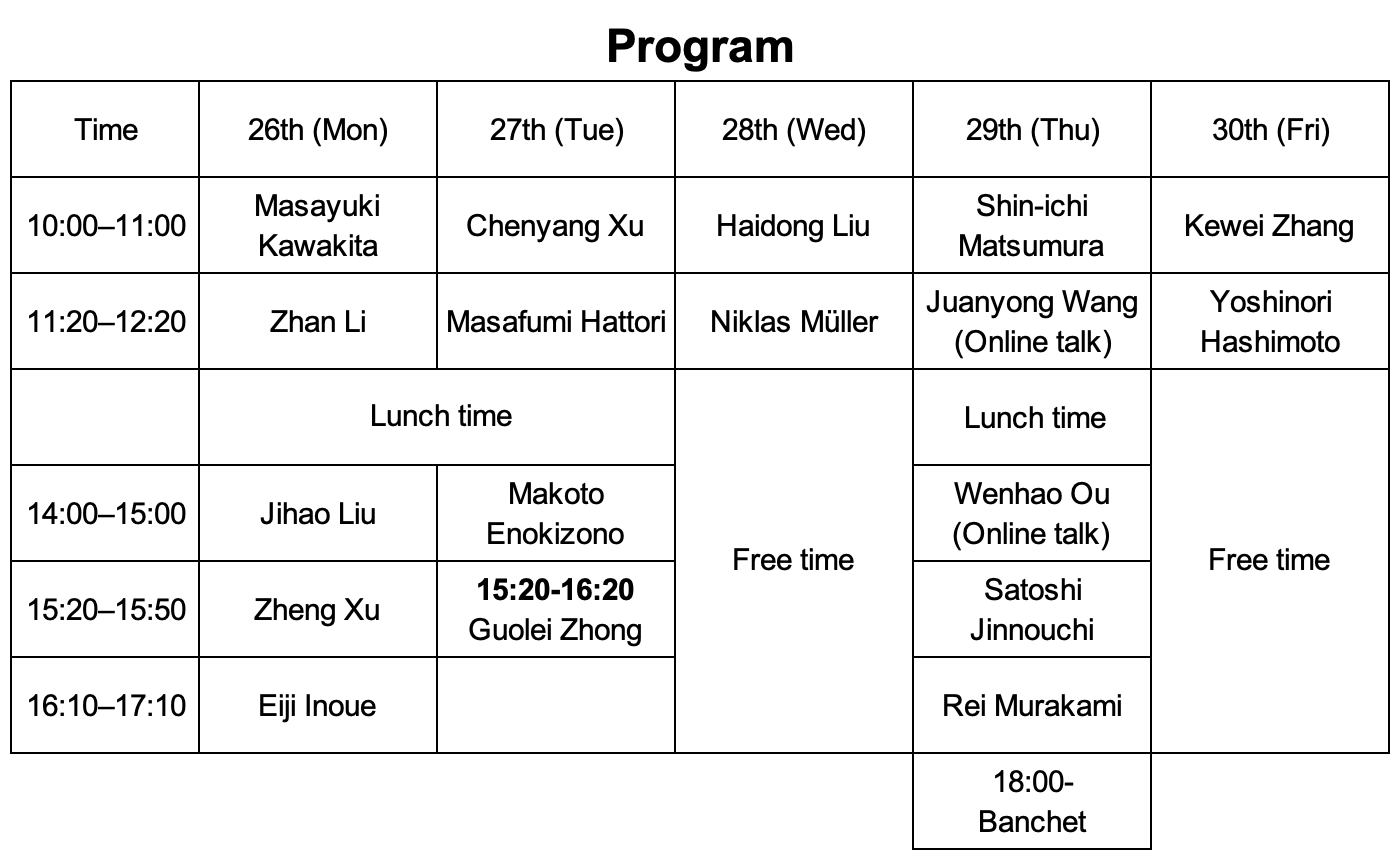
\includegraphics[height=95mm, width=160mm]{program.png}
 %\caption{授業のQRコード}
\end{center}
\end{figure}


%%%%%%%%%%%%%%%%%%%%%%%%%
\begin{comment}

\begin{center}
% ← 表全体の文字サイズを小さくする
\setlength{\tabcolsep}{10pt}
\renewcommand{\arraystretch}{1.5}

\begin{tabular}{|p{1cm}|c|c|c|c|c|}
\hline
      & 26th  & 27th  & 28th  & 29th  & 30th \\ \hline
\shortstack[l]{10:00--\\11:00}   &   &   &   &   &   \\ \hline
\shortstack[l]{11:20--\\12:20}   &   &   &   &   &   \\ \hline
Lunch &   &   &   &   &   \\ \hline
\shortstack[l]{14:00--\\15:00}    &   &   &   &   &   \\ \hline
\shortstack[l]{15:20--\\15:50}  &   &   &   &   &   \\ \hline
\shortstack[l]{16:10--\\17:10}    &   &   &   &   &   \\ \hline
\end{tabular}%
\end{center}
\end{comment}
%%%%%%%%%%%%%%%%%%%%%

  \vskip5mm
  \noindent{\large \bf Organizers}
\begin{itemize}
  \setlength{\parskip}{0cm} 
  \setlength{\itemsep}{0cm}
\item Kento Fujita (The University of Osaka)
\item Kenta Hashizume (Niigata University)
\item Masataka Iwai (The University of Osaka)
  \end{itemize}

\vskip5mm

\noindent{\large \bf Access}

About access, please refer to our homepage
\begin{center}
\url{https://masataka123.github.io/AGCG_Osaka_2026/}
\end{center}


\noindent{\large \bf Supports}

\begin{itemize}
  \setlength{\parskip}{0cm} 
  \setlength{\itemsep}{0cm}
\item 2024 Asian Young Scientist Fellowship (Fujita)
 \item Global Academic Collaboration Program in the University of Osaka. (Iwai)
  \end{itemize}

\newpage
\begin{center}
\noindent{\Large \bf Abstract}
\end{center}
\vskip5mm

\noindent{\large \bf \underline{26th January (Monday)}}
\vskip5mm
\noindent{\bf Masayuki Kawakita (Research Institute for Mathematical Sciences (RIMS), Kyoto University)}\\
Minimal log discrepancies on threefold singularities
\vskip3mm
The minimal log discrepancy is an invariant of singularities.
The ACC for minimal log discrepancies, together with the lower
semi-continuity, will imply the termination of flips. However, the ACC is
still unknown in dimension three, and it is one of the most important
remaining problems in the birational geometry of threefolds. I will
present a proof of this ACC on a fixed threefold.
\vskip8mm

\noindent{\bf Zhan Li (Southern University of Science and Technology (SUSTech))}\\
On the Morrison-Kawamata dream space and its applications
\vskip3mm
I will discuss the theory of Morrison-Kawamata dream spaces, which axiomatizes varieties (not necessarily of Calabi-Yau type) that satisfy the Morrison-Kawamata cone conjecture. If time permits, I will also present some applications of this theory. This talk is based on the joint work with Sung Rak Choi, Xingying Li and Chuyu Zhou.
\vskip8mm

\noindent{\bf Jihao Liu (Peking University)}\\
Birational geometry of algebraically integrable adjoint foliated structures
\vskip3mm
I will discuss recent progress on the birational geometry of algebraically integrable adjoint foliated structures, which can be seen as a structure in between of fibrations and foliations. I will introduce recent developments on this subject (MMP, BAB, abundance, ACC, birational boundedness). Time permitted I will explain why a natural moduli functor for fibrations is expected to be constructed using adjoint foliated structures. The talk is based on a series of works of myself with C. Birkar, P. Cascini, J. Han, Z. Hu, F. Meng, C. Spicer, R. Svaldi, L. Xie, Z. Xu and others.
\vskip8mm

\noindent{\bf Zheng Xu (Peking University)}\\
Abundance conjecture for foliations
\vskip3mm
In this talk, I will discuss the abundance conjecture for foliations. Although abundance for foliations fails even for surfaces, I will explain that a suitable variant of it does hold, assuming the abundance conjecture for varieties. This is a joint work with Jihao Liu.
\vskip8mm

\newpage
\noindent{\bf Eiji Inoue (Kyoto University)}\\
An algebro-geometric entropy formula for MMP with scaling
\vskip3mm
In his celebrated work, Perelman introduced two functionals (F and W) which are monotone along Ricci flow. As an algebro-geometric counterpart of this functional, we introduce mu-entropy of valuation and show its monotonicity along MMP with scaling. We also explain relation to Perelman's functional, Sun-Zhang's weighted volume of Fano fibration and K-stability.
\vskip12mm


\noindent{\large \bf \underline{27th January (Tuesday)}}
\vskip5mm
\noindent{\bf Chenyang Xu (Princeton university)}\\
Properness of K-moduli
\vskip3mm
(Joint with Harold Blum, Yuchen Liu, and Ziquan Zhuang)
We present a new proof of the properness of K-moduli spaces. While our approach still depends on the higher-rank finite generation theorem, it avoids the use of Halpern-Leistner's $\Theta$-stratification theory. Instead, we develop a purely birational method, rooted in a relative framework for K-stability, which provides a more direct geometric proof of properness.
\vskip8mm

\noindent{\bf Masafumi Hattori (University of Nottingham)}\\
Applications of K-moduli of quasimaps to K-moduli conjecture for Calabi-Yau fibrations over curves
\vskip3mm
Odaka proposed the K-moduli conjecture in 2010, predicting the existence of a moduli space of K-polystable objects with an ample CM line bundle. While this conjecture has been solved in the Fano case, it remains open in general. Recent developments of Fine, Dervan-Sektnan and Ortu have highlited the relevance of the existence of cscK metrics and K-stability for 
$(X,\epsilon A+L)$ for sufficiently small $\epsilon$, where $f\colon (X,A)\to (B,L)$ is a fibration. According to their works, such K-stability is closely related to some K-stability of fibers and the bases. Especially in the Calabi-Yau fibration over curve case, uniform K-stability in this context (uniform adiabatic K-stability) coincides with the log twisted K-stability on the base. In this talk, we will regard the base curve as a quasimap and introduce the notion of K-moduli of quasimaps. By using this framework, we address the K-moduli conjecture for Calabi-Yau fibrations over curves whose generic fibers are either Abelian varieties or HyperK\"ahler manifolds. This is a joint work arXiv:2504.21519 with Kenta Hashizume.
\vskip8mm

\newpage

\noindent{\bf Makoto Enokizono (the University of Tokyo)}\\
Normal stable degenerations of Horikawa surfaces
\vskip3mm
Horikawa surfaces are surfaces of general type satisfying the equation $K^2=2p_g-4$, which represents the equality of the Noether inequality $K^2\ge2p_g-4$ for surfaces of general type. In the 1970s, Horikawa conducted a detailed study of smooth Horikawa surfaces, providing a classification of these surfaces and describing their moduli spaces.
In this talk, I will present an explicit classification of normal stable degenerations of Horikawa surfaces. Specifically, I will discuss the following results:
\begin{itemize}
\item[(1)] Classification of Horikawa surfaces with $\mathbb{Q}$-Gorenstein smoothable log canonical singularities.
\item[(2)] Criterion for determining the (global) $\mathbb{Q}$-Gorenstein smoothability of the surfaces described in (1).
\item[(3)] Description of the KSBA moduli spaces for $\mathbb{Q}$-Gorenstein smoothable normal stable Horikawa surfaces.
\end{itemize}
This is joint work with Hiroto Akaike, Masafumi Hattori and Yuki Koto.
\vskip8mm

\noindent{\bf Guolei Zhong (Center for Complex Geometry of Institute for Basic Science (IBS-CCG))}\\
Holomorphic symplectic geometry of elliptic surfaces
\vskip3mm
Let $X$ be a complex surface admitting a nowhere vanishing holomorphic 2-form; such a form induces a holomorphic symplectic structure on $X$. In this talk, we consider the case when $X$ is an elliptic surface and study how the symplectic geometry is related to the underlying complex geometry of the elliptic fibration. Applications will be addressed to the classifications of isogenies of symplectic surfaces. This is based on a joint work with Jun-Muk Hwang.
\vskip8mm

\newpage

\noindent{\large \bf \underline{28th January (Wednesday)}}
\vskip5mm
\noindent{\bf Haidong Liu (Sun Yat-sen University)}\\
A Kawamata-Miyaoka type inequality
\vskip3mm
In the classification of (weak) Fano varieties, Kawamata-Miyaoka type inequalities which concern the relations between the first and the second Chern classes play an important role. In this talk, I will show some recent progress on these inequalities and their application in the classification of terminal/canonical Fano threefolds. Part of these series works is jointed with Masataka Iwai and Chen Jiang, with Jie Liu, with Chen Jiang and Jie Liu.
\vskip8mm

\noindent{\bf Niklas Müller (University of Freiburg)}\\
Inequalities of Miyaoka-type and Uniformisation of Minimal Varieties of Intermediate Kodaira Dimension
\vskip3mm
In this talk we present, for any integers $0 \leq \nu \leq n$, a set of inequalities satisfied by the Chern classes of any minimal complex projective variety of dimension $n$ and numerical dimension $\nu$. In the cases where $\nu$ is either very small or very large compared with $n$, this recovers many previously known results, notably of Miyaoka and others. We demonstrate that these inequalities are sharp by providing an explicit characterisation of those varieties achieving the equality; our proof, in particular, resolves the Abundance conjecture in this situation. This talk is partly based on joint work with Masataka Iwai and Shin-ichi Matsumura.
\vskip12mm




\noindent{\large \bf \underline{29th January (Thursday)}}
\vskip5mm
\noindent{\bf Shin-ichi Matsumura (Tohoku University)}\\
The nonvanishing problem for varieties with nef anticanonical bundle
\vskip3mm
In this talk, I discuss the nonvanishing problem in the framework of the ''generalized'' Minimal Model Program.
I first explain a structure theorem for maximally rationally connected fibrations of Kahler klt pairs with nef anticanonical divisor,
which generalizes Cao-H\"oring's result for smooth projective varieties.
I also show that this structure theorem reduces the nonvanishing problem for nef anticanonical divisors to the rationally connected varieties, and the numerical class of the nef anticanonical bundle of projective 3-folds is represented by an effective divisor.
The first part of this talk is joint work with Juanyong Wang (Chinese Academy of Sciences) and
the latter part is joint work with Thomas Peternell (Bayreuth), Vladimir Lazi\'c, Nikolaos Tsakanikas, Zhixin Xie (Saarbrucken).
\vskip8mm

\newpage 
\noindent{\bf Juanyong Wang (Academy of Mathematics and Systems Science, Chinese Academy of Sciences (AMSS CAS))}\\
Fundamental groups of compact Kähler varieties with nef anti-log canonical divisor
\vskip3mm
It is proved by M. Păun (1997, 2017) that the fundamental group of a compact Kähler manifold is almost Abelian if its anti-canonical bundle is nef, and it is expected that similar results hold for mildly singular Kähler varieties. In this talk, I will explain how we apply the recent development in the theory of Kähler RCD spaces to study this problem. This is an ongoing joint work with Xin Fu, Bin Guo and Jian Song. 
\vskip8mm

\noindent{\bf Wenhao Ou (Academy of Mathematics and Systems Science, Chinese Academy of Sciences (AMSS CAS))}\\
Unitary flat vector bundles on compact K\"ahler varieties 
\vskip3mm
In this talk, we will present a recent joint work with Xin Fu. We prove that a stable reflexive coherent sheaf, on a compact K\"ahler variety with klt singularities, is a unitary flat vector bundle up to quasi-\'etale cover, if and only if its first and second orbifold Chern classes are both zero. 
\vskip8mm

\noindent{\bf Satoshi Jinnouchi (The University of Osaka)}\\
Towards the Kobayashi-Hitchin correspondence for big classes
\vskip3mm
The Kobayashi-Hitchin correspondence asserts the equivalence between the slope stability of holomorphic vector bundles and the existence of the Hermitian-Yang-Mills metrics. In the Kähler setting, the correspondence has been well-established and its extension beyond Kähler case has attracted significant interest. In this talk, I firstly present the formulation of the correspondence on compact complex manifolds with big classes. The analysis in the big-class setting is highly challenging in general, since metrics representing big classes are merely closed positive (1,1)-currents. I will then present a version of the correspondence with respect to Kähler currents, which provides a partial result toward the full generalization.
\vskip6mm

\noindent{\bf Rei Murakami (Tohoku University)}\\
An analytic proof of Griffiths' conjecture on compact Riemann surfaces
\vskip3mm
Griffiths conjecture asserts that the ampleness of a holomorphic vector bundle is equivalent to the existence of a Hermitian metric with Griffiths positive curvature. In the case of line bundles, this is a consequence of Kodaira's embedding theorem, and the conjecture is also settled in dimension one. Recently, J.-P. Demailly proposed an analytic approach to this conjecture based on a system of partial differential equations. In this talk, we present a new proof of the one-dimensional case of Griffiths' conjecture using this method. The results in this talk are based on arXiv:2509.23201.

\newpage

\noindent{\large \bf \underline{30th January (Friday)}}
\vskip5mm
\noindent{\bf Kewei Zhang (Beijing Normal University)}\\
Regularizing the entropy in K\"ahler geometry
\vskip3mm
Searching for constant scalar curvature metrics on compact Kahler manifolds is one of the central problems in geometric analysis. Recent work of Chi Li reduces this problem to Boucksom-Jonsson's regularization conjecture for the entropy. We will first review Li's work, which relies on non-Archimedean techniques. Then we present some new progress on this problem, by using pluripotential theory and quantization techniques. This talk is based on my recent joint work with T. Darvas.
\vskip8mm

\noindent{\bf Yoshinori Hashimoto (Osaka Metropolitan University)}\\
Coupled Kähler-Einstein metrics and coupled Ding stability 
\vskip3mm
A foundational theorem in Kähler geometry states that a Kähler-Einstein metric exists on a Fano manifold (with discrete automorphisms) if and only if it is uniformly Ding stable. When Kähler-Einstein metrics do not exist, we can seek coupled Kähler-Einstein metrics, introduced by Hultgren and Witt Nyström, defined in terms of decompositions of the anticanonical bundle. The main result of this talk is the equivalence between the coupled uniform Ding stability (as appropriately defined) and the existence of coupled Kähler-Einstein metrics. Time permitting, we also discuss another equivalent condition involving the stability threshold and its coupled version. This is a joint work with Kento Fujita.
\vskip8mm




\end{document}